\section{Grid orthogonality, uniformity and skewness}
\label{sec:theory:skewness}

A grid without orography may be orthogonal, uniform, and have no skewness, and these properties simplify the spatial discretisation.  However, in the presence of terrain, most methods alter the shape of grid cells to better represent the surface.  With the exception of the full-step shaving method, these cell modifications will affect orthogonality, uniformity and skewness.

A uniform grid is one in which cell dimensions are uniform \autocite{leveque2002}.  On a $x$--$z$ plane, this means that $\Delta x$ and $\Delta z$ are constant.  When linearly interpolating onto a cell face, a uniform grid results in second-order accuracy because the centre of the face is equidistant from the two adjoining cell centres.  On a non-uniform grid, the interpolation becomes first-order accurate.

A grid is orthogonal when angles between cell vertices are \ang{90}; that is, when cells are rectangular.  Piecewise linear cut cell grids are orthogonal everywhere except where cells intersect the ground, whereas terrain following grids tend to have greater non-orthogonality.

\begin{figure}
	\captionsetup[subfigure]{position=b}
	\centering
	\subcaptionbox{Orthogonal grid \label{fig:theory:skewness:ortho}}[0.49\textwidth]{\documentclass[tikz]{standalone}
\usepackage{bm}
\newcommand{\vect}{\bm}
\newcommand{\del}{\boldsymbol{\nabla}}

\begin{document}
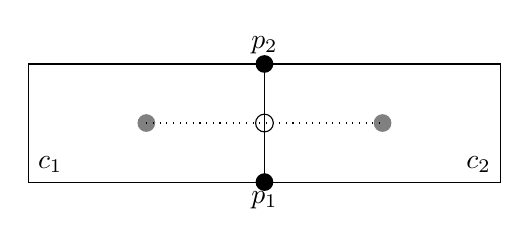
\begin{tikzpicture}[
  scale=0.75,
  cpnt/.style={fill=gray},
  vertex/.style={fill=black},
  arr/.style={thick, <->},
  mag/.style={dashed, thick, <->}
]
\draw (0,0) rectangle (4,2);
\draw (4,2) -- (8,2) -- (8,0) -- (4,0);
\path [vertex] (4,0) circle [radius=0.15] node [below] {$p_1$};
\path [vertex] (4,2) circle [radius=0.15] node [above] {$p_2$};
\node [above right] at (0,0) {$c_1$};
\node [above left] at (8,0) {$c_2$};

\path [cpnt] (2,1) circle [radius=0.15];
\path [cpnt] (6,1) circle [radius=0.15];
\draw [dotted] (2,1) -- (6,1);
\draw (4,1) circle [radius=0.15];
\end{tikzpicture}
\end{document}
\vspace{1em}}
	\hfill
	\subcaptionbox{Non-orthogonal grid \label{fig:theory:skewness:nonortho}}[0.49\textwidth]{\documentclass[tikz]{standalone}
\usepackage{bm}
\newcommand{\vect}{\bm}
\newcommand{\del}{\boldsymbol{\nabla}}

\begin{document}
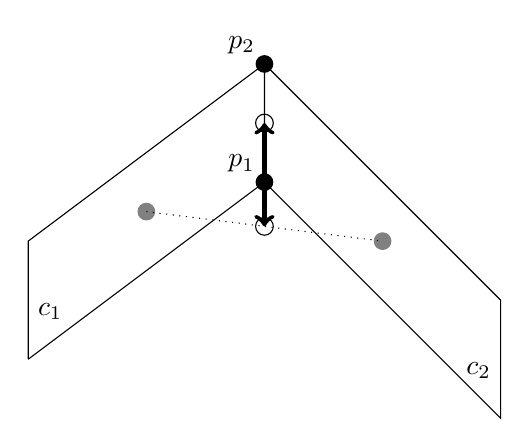
\begin{tikzpicture}[
  scale=0.75,
  cpnt/.style={fill=gray},
  vertex/.style={fill=black},
  arr/.style={ultra thick, <->},
  mag/.style={dashed, thick, <->}
]
\draw (0,0) -- (4,3) -- (4,5) -- (0,2) -- (0,0);
\draw (4,3) -- (8,-1) -- (8,1) -- (4,5);
\node [above right] at (0,0.5) {$c_1$};
\node [above left] at (8,-0.5) {$c_2$};

\path [vertex] (4,3) circle [radius=0.15] node [above left] {$p_1$};
\path [vertex] (4,5) circle [radius=0.15] node [above left] {$p_2$};

\path [cpnt] (2,2.5) circle [radius=0.15];
\path [cpnt] (6,2) circle [radius=0.15];

\draw (4,4) circle [radius=0.15];
\draw (4,2.25) circle [radius=0.15];
\draw [dotted] (2,2.5) -- (6,2);
\draw [arr] (4,4) -- (4,2.25);
\end{tikzpicture}
\end{document}
}
%
	\caption{Skewness measurements on two-cell grids.  Cell centres are represented by grey circles, and face vertices by filled black circles.  The face centre and the intercept with the dotted line that joins the cell centres are denoted by open circles.  In the orthogonal grid (\subcaptionref{fig:theory:skewness:ortho}), skewness is zero.  In the non-orthogonal grid (\subcaptionref{fig:theory:skewness:nonortho}), the skewness is measured by the double-ended arrow.}
	\label{fig:theory:skewness}
\end{figure}

Non-orthogonality typically causes skewness, which is the misalignment of cell faces with adjoining cell centres.
Consider a two dimensional grid having two cells, $c_1$ and $c_2$ that share a common face $f$ having vertices $p_1$ and $p_2$.  Skewness is defined as the distance between the centre of face $f$, and the intercept of a line connecting the centres of $c_1$ and $c_2$ with the line passing through points $p_1$ and $p_2$ \autocite{moraes2013}.

In an orthogonal grid, seen in figure~\ref{fig:theory:skewness:ortho}, the skewness is zero.  Skewness increases when the grid becomes non-orthogonal, as shown in figure~\ref{fig:theory:skewness:nonortho}.  If high accuracy is required, a numerical scheme must account for this skewness when interpolating values at cell centres onto a cell face.
